\documentclass[12pt]{article}
%Gummi|065|=)
\usepackage{amsmath, amsfonts, amssymb}
\usepackage[margin=0.5in]{geometry}
\usepackage{xcolor}
\usepackage{graphicx}
\newcommand{\off}[1]{}
\DeclareMathSizes{20}{30}{21}{18}

\newcommand{\myhrule}{}

\usepackage{tikz}

\title{\textbf{ Examples:  Pythagorean Theorem }}
\author{John D Mangual}
\date{}
\begin{document}

\fontfamily{qag}\selectfont \fontsize{25}{30}\selectfont

\maketitle

\noindent At this stage of the game, I have felt a need to review the Pythagorean theorem.  
$$ a^2 + b^2 = c^2 $$
Sadly I can't think of any really good examples, but we do get our first irrational number:
$$ \sqrt{1^2 + 1^2 } = \sqrt{2}$$
This is the hypoteneus lenght of an isosceles right triangle:
\begin{center}
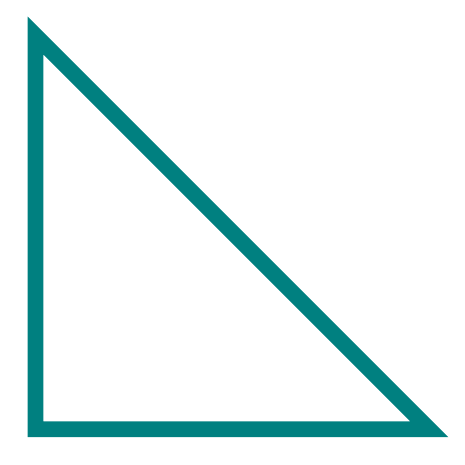
\begin{tikzpicture}
\draw[color=blue!50!green, line width=2mm] (0,0)--(5,0)--(0,5)--cycle;
\end{tikzpicture}
\end{center}
and we can expend some effort showing that $\sqrt{2} \neq \frac{p}{q}$ for some intgers $p, q \in \mathbb{Z}$.
\newpage

\noindent For something more contemporary, Alex Kontrovich shows us that all Pythagorean triples can be written:
$$ x = u^2 - v^2, \; y = 2uv\; z = u^2 + v^2 $$
and shows us a homomorphism $\text{SL}_2(\mathbb{R}) \to \text{SO}(2,1) $
$$ \left( \begin{array}{cc} 
a & b \\ c & d\end{array}\right) 
\mapsto 
\left( \begin{array}{ccc} 
\frac{a^2 - b^2 - c^2 + d^2}{2} & ac -bd & 
\frac{a^2 - b^2 + c^2 - d^2}{2} \\
ab - cd & bc + ad & ab + cd \\
\frac{a^2 + b^2 - c^2 - d^2}{2} & 
ac + bd & \frac{a^2 + b^2 + c^2 + d^2}{2}
\end{array}\right)$$
Several things jump out at me about this formula:
\begin{itemize}
\item We get all possible quadratic forms in $a,b,c,d$ that are ``invariant" or at least transform nicely\footnote{In mathematics ``good" means ``I just made up a word.  Figure it out for yourself."} such as $a^2 - b^2 - c^2 + d^2$
\item $SO(2,1)$ preserves $x^2 +y^2 - z^2=0$ which is the ``light cone" in special relativity, and also the hyperboloid\footnote{These days one might consider $x^2 +y^2 - z^2 - w^2 = 1$.  Especially if you are Juan Maldacena.} of one sheet $x^2 + y^2 - z^2 = 1$.
\item Since $\text{SL}(2, \mathbb{Z})$ is generated by $z \mapsto z+1$ and $z \mapsto - \frac{1}{z}$, the Pythagorean triples form a ``tree"
\item It may be reasonable\footnote{How about something unreasonable: $\text{GL}_2(\mathbf{A})$ if you know what \textbf{ad\`{e}les}  are.} to examine $\text{SL}(\mathbb{Z}[i])$ or the equation $x^2 + y^2 - \sqrt{2}z^2 < 10^{-6}$.
\end{itemize}

\newpage


\noindent Kontrovich's question (or possibly Hee Oh's) is how many factors in :
$$ \frac{1}{2}xy = \frac{A}{6} = \frac{1}{6}(u+v)(u-v)\, uv$$
When does this Area have at $\leq$ 4 factors\footnote{This is as close as we can get to prime. I am not going to give you an answer.  How might we use such a Pythagorean triple?  The proofs use the most difficult techniques in mathematics.  I am curious what you can obtain with less\dots} ? \\ \\
Just a reminder why quadratic quations are everywhere:
\begin{eqnarray*} f(x+t) &=& e^{t\,\frac{d}{dx}} f(x) \\ 
&=& \left[1 + t\;\frac{d}{dx} + \frac{t^2}{2!} \frac{d^2}{dx^2} + \frac{t^3}{3!} \frac{d^3}{dx^3}+ \dots \right]f(x) \\  \\
&=& f(x) + tf'(x) + (t^2/2)f''(x) + \dots \end{eqnarray*}
If it happens that $f'(x) = 0$ then $\deg f \approx 2$:
$$ f(x+t) = f(x) +  \tfrac{1}{2}f''(x)\;t^2 + \dots $$
By the \textbf{Fundamental Theorem of Algebra} there should be $\approx 2$ roots $f(x) = 0$ with $x \in \mathbb{C}$.
$$ f(x + s, y + t) \approx
f(x,y) + \frac{1}{2}\left[ 
s^2 \,\frac{\partial^2 f}{\partial x^2}+
2st \,\frac{\partial f}{\partial x}\frac{\partial f}{\partial y}+
t^2 \,\frac{\partial^2 f}{\partial y^2}
\right] $$
In two dimensions.  

\newpage

\noindent How about some more exotic examples of the quadratic equation? \\ \\
Here is an estimate of the Laplacian I have always liked:
$$ \Delta \approx \frac{1}{h^2(w+2)}
\left[ \begin{array}{ccc}
1 & w & 1 \\
w & -4(w+1) & w \\
1 & w & 1 \end{array} \right] $$
This construction is connected to the Vernose map (or Veronese embedding\footnote{Recall that $5+1 = 2 \times (2+1)$.}):
$$(u:v:w) \in \mathbb{P}^2 \mapsto (u^2 : v^2: w^2 : uv: vw: uw\in \mathbb{P}^5 $$
these are called Sobel masks.  I lost my copy of \textbf{Robot Vision}.  Here we recover:
$$
\frac{1}{8h} \left[ 
\begin{array}{ccc} 
1 & 4 & 1 \\ 4 & -20 & 4 \\ 1 & 4 & 1\end{array}
\right]
= \Delta + \frac{h^2}{12} \Delta^2 + O(h^4)
 $$
 as $h \to 0$.  The idea is to approximate a linear functional\footnote{Not function, function\textit{al}\dots} as a sum of points:
$$ \Delta f( \vec{v}) \approx 
\sum_{P \in \square } w_i \, f(\vec{v} + \vec{P}) $$
That's the (truly terrible) approximation I always use\footnote{These are refined versions of Taylor's Theorem.  Or the mean value theorem $f(b) - f(a) \approx f'(c)(b-a)$ for $a < c < b$.}. 

\newpage

\noindent The Veronese map is used to lift approximations of $\nabla$ to other higher-order operators.  They are a special case of:
$$(x,y) = (\cos \theta, \sin \theta) 
\mapsto (x^2 - y^2, 2xy) = (\cos 2\theta, \sin 2\theta) $$
this is the \textbf{Harmonic} Veronese map.  The same paper also show integral version:
$$ \frac{1}{4\pi} \int_{S^2} F \cdot dS 
\approx \frac{1}{12} \sum_{P \in M} F(P) $$
where $M = (\pm 1, \pm 1, 0)\text{ or } (\pm 1, 0, \pm 1)\text{ or }(0, \pm 1, \pm 1)$ \\ forming the vertices of a \textbf{snub cube}.

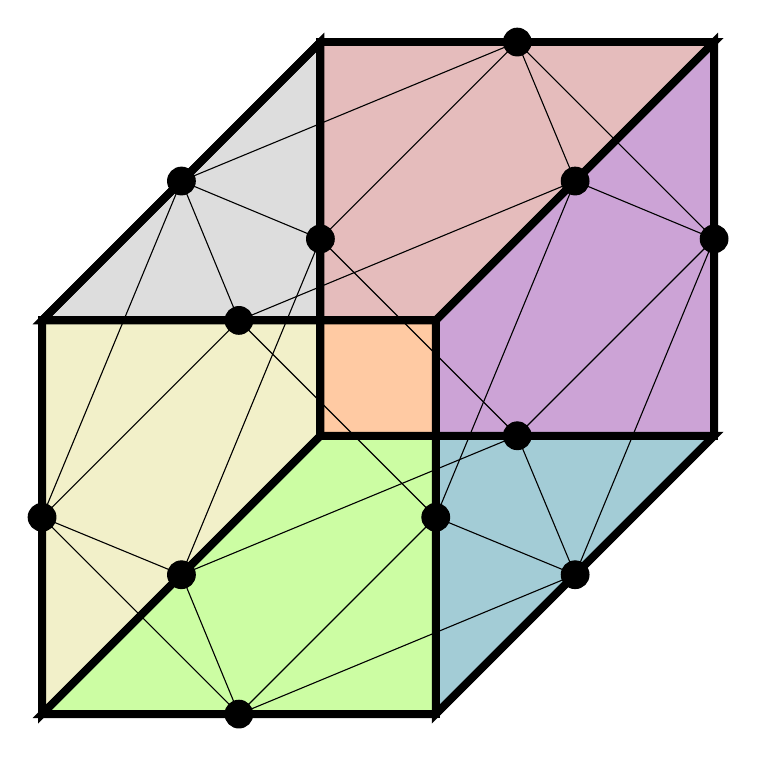
\begin{tikzpicture}[scale=5]
% draw some points
\node[coordinate] (A) at (0,0) {};
\node[coordinate] (B) at (1,0) {};
\node[coordinate] (C) at (1,1) {};
\node[coordinate] (D) at (0,1) {};
\node[coordinate] (E) at (0.707,0.707) {};
\node[coordinate] (F) at (1.707,0.707) {};
\node[coordinate] (G) at (1.707,1.707) {};
\node[coordinate] (H) at (0.707,1.707) {};

% draw some lines
\draw[fill=yellow, opacity=0.2] (A)--(B)--(C)--(D)--cycle;
\draw[fill=red, opacity=0.2] (E)--(F)--(G)--(H)--cycle;
\draw[fill=green, opacity=0.2] (A)--(B)--(F)--(E)--cycle;
\draw[fill=blue, opacity=0.2] (B)--(F)--(G)--(C)--cycle;
\draw[fill=black!50!white, opacity=0.2] (D)--(C)--(G)--(H)--cycle;
\draw[fill=black!25!white, opacity=0.2] (A)--(E)--(H)--(D)--cycle;

\draw[line width=0.1cm] (A)--(B)--(C)--(D)--cycle;
\draw[line width=0.1cm] (E)--(F)--(G)--(H)--cycle;
\draw[line width=0.1cm] (A)--(B)--(F)--(E)--cycle;
\draw[line width=0.1cm] (B)--(F)--(G)--(C)--cycle;
\draw[line width=0.1cm] (D)--(C)--(G)--(H)--cycle;
\draw[line width=0.1cm] (A)--(E)--(H)--(D)--cycle;

\node[coordinate] (a) at (0.5,0) {};
\node[coordinate] (b) at (1,0.5) {};
\node[coordinate] (c) at (0.5,1) {};
\node[coordinate] (d) at (0,0.5) {};

\node[coordinate] (e) at (1.354,0.354) {};
\node[coordinate] (f) at (1.354,1.354) {};
\node[coordinate] (g) at (0.354,1.354) {};
\node[coordinate] (h) at (0.354,0.354) {};

\node[coordinate] (i) at (1.207,0.707) {};
\node[coordinate] (j) at (1.707,1.207) {};
\node[coordinate] (k) at (1.207,1.707) {};
\node[coordinate] (l) at (0.707,1.207) {};

\draw[fill=black] (a) circle (1pt);
\draw[fill=black] (b) circle (1pt);
\draw[fill=black] (c) circle (1pt);
\draw[fill=black] (d) circle (1pt);

\draw[fill=black] (e) circle (1pt);
\draw[fill=black] (f) circle (1pt);
\draw[fill=black] (g) circle (1pt);
\draw[fill=black] (h) circle (1pt);

\draw[fill=black] (i) circle (1pt);
\draw[fill=black] (j) circle (1pt);
\draw[fill=black] (k) circle (1pt);
\draw[fill=black] (l) circle (1pt);

\draw (a)--(b)--(c)--(d)--cycle;
\draw (i)--(j)--(k)--(l)--cycle;
\draw (e)--(j)--(f)--(b)--cycle;
\draw (d)--(h)--(l)--(g)--cycle;
\draw (a)--(e)--(i)--(h)--cycle;
\draw (c)--(f)--(k)--(g)--cycle;

\end{tikzpicture} \\
Janos Kollar gives us a bunch of exotic new Veronese embeddings.  

\newpage

\fontfamily{qag}\selectfont \fontsize{12}{10}\selectfont

\begin{thebibliography}{}


\item Terence Tao.  \textbf{Determinantal Processes} \\ \texttt{https://terrytao.wordpress.com/2009/08/23/determinantal-processes/}

\item Alex Kontrovich, Hee Oh \textbf{
Almost prime Pythagorean triples in thin orbits}
\texttt{arXiv:1001.0370}


\item Alexander Belyaev, Boris Khesin, Serge Tabachnikov. \textbf{Discrete spherical means of directional derivatives and Veronese maps.}
\texttt{arXiv:1106.3691}

\end{thebibliography}


\end{document}